






\documentclass[10pt]{article}
\usepackage[preprint]{tmlr}
\usepackage{amsmath,amssymb,booktabs,graphicx,xcolor,hyperref,caption}
\captionsetup{font=small}
\renewcommand{\cite}{\citep}
\newcommand{\pending}[1]{\textcolor{red}{[#1]}}
% GENERATED by research/w6_figures.py from research/outputs/*.json -- do not edit
\newcommand{\HFullLstmHalf}{$-60.7$~[$-71.4$, $-50.5$]}
\newcommand{\HFullMlpTest}{$-28.3$~[$-39.0$, $-16.7$]}
\newcommand{\HFullMtdHalf}{$-55.3$~[$-65.7$, $-45.2$]}
\newcommand{\HFullOne}{$-75.4$~[$-88.1$, $-60.8$]}
\newcommand{\HFullZero}{$-63.2$~[$-75.5$, $-50.4$]}
\newcommand{\HStateMtdHalf}{$-51.6$~[$-62.5$, $-41.7$]}
\newcommand{\HStateOne}{$-55.2$~[$-68.1$, $-42.9$]}
\newcommand{\HStateZero}{$-49.0$~[$-60.1$, $-39.4$]}
\newcommand{\MOneBCostHigh}{$-208.9$~[$-255.3$, $-162.3$]}
\newcommand{\MOneBCostLow}{$-82.5$~[$-96.6$, $-68.5$]}
\newcommand{\MOneBExpCut}{72\%}
\newcommand{\MOneBHighMax}{+301}
\newcommand{\MOneBHighMin}{+92}
\newcommand{\MOneBMedMtd}{266}
\newcommand{\MOneBMedThr}{196}
\newcommand{\MOneBMiss}{$-5.6$~[$-13.9$, $+2.4$]}
\newcommand{\MOneBPStarHigh}{above 0.6}
\newcommand{\MOneBPStarLowMax}{0.49}
\newcommand{\MOneBPStarLowMin}{0.36}
\newcommand{\MOneBTailCens}{29\%}
\newcommand{\MOneCBurdenCostly}{4.5}
\newcommand{\MOneCBurdenNoCost}{18\%}
\newcommand{\MOneCCostOneLow}{$-9.9$~[$-22.5$, $+7.6$]}
\newcommand{\MOneCHighFour}{$+62.3$~[$+36.9$, $+90.0$]}
\newcommand{\MOneCHighOne}{$-137.8$~[$-166.2$, $-112.6$]}
\newcommand{\MOneCHighThree}{$+34.0$~[$+4.5$, $+57.7$]}
\newcommand{\MOneCHighTwo}{$-29.4$~[$-48.1$, $-2.0$]}
\newcommand{\MOneCostHigh}{$-76.6$~[$-88.6$, $-64.7$]}
\newcommand{\MOneCostLow}{$-25.5$~[$-31.2$, $-20.0$]}
\newcommand{\MOneMiss}{$+38.5$~[$+36.1$, $+41.0$]}
\newcommand{\MOnePStarHighMax}{0.50}
\newcommand{\MOnePStarHighMin}{0.23}
\newcommand{\MOnePStarLowMax}{0.26}
\newcommand{\MOnePStarLowMin}{0.10}
\newcommand{\MOneRegMax}{+123}
\newcommand{\MOneRegMin}{+13}
\newcommand{\POneLstmMtd}{$-1.0$~[$-12.8$, $+10.0$]}
\newcommand{\POneN}{55}
\newcommand{\POneOdeLstm}{$-2.4$~[$-28.1$, $+27.7$]}
\newcommand{\POneOdeMlp}{$-44.0$~[$-59.5$, $-30.5$]}
\newcommand{\POneOdeMtd}{$-13.2$~[$-33.2$, $+3.3$]}
\newcommand{\RTwoExcl}{12}
\newcommand{\RTwoMWp}{0.04}
\newcommand{\RTwoN}{67}
\newcommand{\RTwoPearson}{$-0.73$}
\newcommand{\RuleHalfProvisional}{0.85}
\newcommand{\RuleHalfStrobl}{0.71}
\newcommand{\SAMemOne}{$-44.1$~[$-64.8$, $-30.1$]}
\newcommand{\SAMemZero}{$-42.0$~[$-66.7$, $-26.0$]}
\newcommand{\SAOdeLstmOne}{$-5.9$~[$-27.9$, $+19.9$]}
\newcommand{\SAOdeLstmZero}{$-8.4$~[$-35.8$, $+25.0$]}
\newcommand{\SAOdeMlpOne}{$-50.0$~[$-63.5$, $-37.9$]}
\newcommand{\SAOdeMlpZero}{$-50.4$~[$-65.7$, $-36.2$]}
\newcommand{\SAULstmOne}{170.9}
\newcommand{\SAULstmZero}{240.0}
\newcommand{\SAUMlpOne}{215.0}
\newcommand{\SAUMlpZero}{282.0}
\newcommand{\SAUMtdOne}{162.2}
\newcommand{\SAUMtdZero}{241.6}
\newcommand{\SAUOdeOne}{165.0}
\newcommand{\SAUOdeZero}{231.6}
\newcommand{\SAUThrOne}{214.9}
\newcommand{\SAUThrZero}{282.8}
\newcommand{\SBFb}{$+5.4$~[$-3.5$, $+13.6$]}
\newcommand{\SBFbBest}{LSTM}
\newcommand{\SBFbLstm}{$+5.4$~[$-3.5$, $+13.6$]}
\newcommand{\SBFbLstmDt}{$-16.3$~[$-29.4$, $-4.3$]}
\newcommand{\SBFbMlp}{$-36.0$~[$-44.0$, $-28.0$]}
\newcommand{\SBFbOde}{$-17.7$~[$-39.7$, $0.0$]}
\newcommand{\SBGraceLstm}{$-20.3$~[$-33.9$, $-8.3$]}
\newcommand{\SBGraceLstmDt}{$-5.2$~[$-22.7$, $+9.4$]}
\newcommand{\SBGraceMlp}{$+38.9$~[$+26.7$, $+48.8$]}
\newcommand{\SBOdeLstm}{$-16.1$~[$-37.7$, $+2.3$]}
\newcommand{\SBOdeLstmDt}{$-1.7$~[$-25.2$, $+17.7$]}
\newcommand{\SBOdeMlp}{$-5.4$~[$-24.3$, $+9.3$]}
\newcommand{\SBOdeMtd}{$-13.5$~[$-33.0$, $+2.3$]}
\newcommand{\SBULstmDtFifth}{234.4}
\newcommand{\SBULstmDtHalf}{225.5}
\newcommand{\SBULstmDtZero}{233.2}
\newcommand{\SBULstmFifth}{241.4}
\newcommand{\SBULstmHalf}{247.2}
\newcommand{\SBULstmZero}{232.5}
\newcommand{\SBUMlpFifth}{261.5}
\newcommand{\SBUMlpHalf}{205.7}
\newcommand{\SBUMlpZero}{280.9}
\newcommand{\SBUMtdFifth}{241.8}
\newcommand{\SBUMtdHalf}{241.8}
\newcommand{\SBUMtdZero}{241.8}
\newcommand{\SBUOdeFifth}{232.4}
\newcommand{\SBUOdeHalf}{224.0}
\newcommand{\SBUOdeZero}{236.7}
\newcommand{\SBUThrFifth}{247.5}
\newcommand{\SBUThrHalf}{158.6}
\newcommand{\SBUThrZero}{283.9}
\newcommand{\SThreeBudgetFull}{$+29.0$~[$+11.3$, $+47.1$]}
\newcommand{\SThreeBudgetMlp}{$+7.2$~[$+5.3$, $+9.3$]}
\newcommand{\SThreeFull}{$-41.4$~[$-53.9$, $-27.6$]}
\newcommand{\SThreeFullOne}{$-51.5$~[$-64.7$, $-36.8$]}
\newcommand{\SThreeR}{$-2.8$}
\newcommand{\SThreeRPos}{14/40}
\newcommand{\SThreeUMlpZero}{289.2}
\newcommand{\SThreeUThrZero}{282.8}
\newcommand{\TOneFull}{$-19.6$~[$-25.2$, $-14.7$]}
\newcommand{\TOneR}{$+2.07$}
\newcommand{\TOneRPos}{19/40}
\newcommand{\TOneStepFull}{$+22.0$~[$+9.7$, $+34.1$]}
\newcommand{\TOneStepMlp}{$+0.2$~[$-0.7$, $+1.2$]}
\newcommand{\WBFb}{$-29.1$~[$-55.8$, $-8.2$]}
\newcommand{\WBFbBest}{ODE-RNN}
\newcommand{\WBFbLstm}{$-55.8$~[$-81.5$, $-29.0$]}
\newcommand{\WBFbLstmDt}{$-63.1$~[$-92.4$, $-35.7$]}
\newcommand{\WBFbMlp}{$-40.2$~[$-49.3$, $-30.7$]}
\newcommand{\WBFbOde}{$-29.1$~[$-55.8$, $-8.2$]}
\newcommand{\WBGraceLstm}{$-3.1$~[$-12.8$, $+6.8$]}
\newcommand{\WBGraceLstmDt}{$+17.4$~[$+0.2$, $+36.6$]}
\newcommand{\WBGraceMlp}{$+29.0$~[$+19.2$, $+38.4$]}
\newcommand{\WBOdeLstm}{$+25.7$~[$-13.0$, $+56.4$]}
\newcommand{\WBOdeLstmDt}{$+22.2$~[$+0.8$, $+43.2$]}
\newcommand{\WBOdeMlp}{$-6.1$~[$-34.7$, $+12.9$]}
\newcommand{\WBOdeMtd}{$-23.7$~[$-47.5$, $-5.8$]}
\newcommand{\WBULstmDtFifth}{228.8}
\newcommand{\WBULstmDtHalf}{194.4}
\newcommand{\WBULstmDtZero}{240.7}
\newcommand{\WBULstmFifth}{214.6}
\newcommand{\WBULstmHalf}{201.7}
\newcommand{\WBULstmZero}{216.7}
\newcommand{\WBUMlpFifth}{262.6}
\newcommand{\WBUMlpHalf}{217.3}
\newcommand{\WBUMlpZero}{280.7}
\newcommand{\WBUMtdFifth}{257.6}
\newcommand{\WBUMtdHalf}{257.6}
\newcommand{\WBUMtdZero}{257.6}
\newcommand{\WBUOdeFifth}{239.2}
\newcommand{\WBUOdeHalf}{228.5}
\newcommand{\WBUOdeZero}{245.5}
\newcommand{\WBUThrFifth}{250.1}
\newcommand{\WBUThrHalf}{189.3}
\newcommand{\WBUThrZero}{279.2}
\newcommand{\WCMemOne}{$-82.9$~[$-106.8$, $-58.7$]}
\newcommand{\WCMemZero}{$-73.5$~[$-100.3$, $-48.2$]}
\newcommand{\WCOdeLstmOne}{$-15.7$~[$-43.0$, $+21.8$]}
\newcommand{\WCOdeLstmZero}{$-16.7$~[$-45.7$, $+24.2$]}
\newcommand{\WFiveHfTtp}{7}
\newcommand{\WFiveKzMtdCens}{100\%}
\newcommand{\WFiveKzThrMax}{42}
\newcommand{\WFiveKzThrMin}{28}


\title{Neither Memory nor an ODE-RNN: A Pre-Registered Negative Result\\
for Learned Adaptive-Therapy Policies under Burden-Only Observation}
\author{\name AUTHOR NAME \email AUTHOR@EMAIL \\ \addr AFFILIATION}

\begin{document}
\maketitle

\begin{abstract}
Adaptive therapy tries to keep drug-sensitive tumour cells alive so that they
hold resistant cells in check. Reinforcement learning has been used to schedule
it, and recurrent or continuous-time policies are natural candidates when the
clinician sees only the total tumour burden. We ask whether a policy whose
hidden state is an ODE (an ODE-RNN) schedules better than an LSTM or a
memoryless network, in a virtual-patient simulator, with the main hypotheses and
kill criteria written down before the runs. It does not. Trained by the same
algorithm (PQN), a memoryless network that learns a burden threshold matches or
beats both recurrent networks across patient ranges, under a parameter shift,
and when visits are missed. The task is not trivial, since a per-patient search
on the true simulator finds better schedules, but most of that gap does not
come from memory, and it is smaller than what training the recurrent networks
costs. Cloning a threshold teacher shows that the recurrent networks can
represent a good policy and that PQN fine-tuning then damages them, which
points to the trainer, not the architecture, as the bottleneck for memory in
this setting.
Along the way we identify evaluation pitfalls that can turn a spurious
difference between architectures into an apparently significant one, and we
propose a set of controls for comparisons under partial observation.
\end{abstract}

\section{Introduction}
Adaptive therapy treats a tumour so that drug-sensitive cells survive and keep
competing with resistant ones, instead of trying to eradicate everything. The
idea comes from evolutionary models of resistance, and its first clinical test
in prostate cancer paused and restarted the drug according to the PSA level
\cite{zhang2017}. Whether a rule that simple is the best one is an open
question, and it is a natural place to ask what a learned policy can add.

Reinforcement learning (RL) has been applied to exactly this. On a
Lotka--Volterra (LV) model where the policy sees only total burden, A3C learns a
treat-above-threshold rule close to the clinical algorithm \cite{gallagher2024}.
Recurrent policies are reported to help chemotherapy control when part of the
state is hidden \cite{kiram2026}. Policies fitted to patient data are starting
to appear as well \cite{lu2024}. In these studies the architecture of the policy
is mostly a fixed choice, and the comparison between architectures is not the
question.

That comparison matters because of a common argument. A tumour is a continuous
process observed at irregular visits, so a policy whose hidden state is itself
an ODE \cite{rubanova2019} should carry the right inductive bias, especially
when the biology shifts or visits are missed. The evidence for continuous-time
networks comes mostly from prediction on irregularly sampled series. To our knowledge
there is no controlled test of the argument for control under partial
observation, where the policy also has to learn from reward. Adaptive therapy is a small test bed
for it, because the simulator lets us compare any policy with the true state.

We run that test for one continuous-time design, the ODE-RNN. The main hypotheses and kill criteria were written down before the runs,
so that a null result could not be explained away afterwards; analyses chosen
after seeing results are marked as such. The ODE-RNN is compared with a memoryless MLP,
an LSTM and an LSTM that is told the gap between visits, all trained with the
same algorithm and matched in size. The ODE-RNN never beats the best discrete
arm. The obvious objection is that recurrent networks are simply hard to train,
so we address it in two ways: a search on the true simulator that measures how
much room there is for memory at all, and a warm-start experiment that asks
whether the recurrent networks can represent a good policy and lose it in
training.

This paper makes three contributions.
\begin{enumerate}
\item A controlled comparison. One trainer, one environment and one evaluation
protocol, with only the Q-network swapped and the recurrent arms matched in size.
\item A negative result and a partial explanation. There is no ODE-RNN edge in
range, under a parameter shift or with missed visits. The headroom split and the
warm-start experiment suggest that the recurrent deficit is a learning cost of
PQN, with little room for memory to repay it.
\item A record of how the result was reached: four evaluation mistakes that
produced a wrong result that looked publishable, the controls that found them,
and a table of every registered run.
\end{enumerate}
We do not claim that no memory policy could help, that no other trainer would
avoid the deficit (two others did not let a reference beat the memoryless
network, so they cannot test it), or anything about real patients; all patients are simulated.

\section{Related work}
\paragraph{RL for tumour control.} Learned dosing policies on tumour ODEs have
been reported to approach a clinical threshold rule from burden alone
\cite{gallagher2024}, to approach an optimal-control benchmark when every
subpopulation is observed \cite{kidane2026}, to benefit from recurrence when part
of the state is hidden \cite{kiram2026}, and to prolong time to progression on
models fitted to trial patients \cite{lu2024}. None compares memory with
continuous time under one trainer, with uncertainty over training seeds. Optimal
control gives a useful contrast: when the drug raises the mutation rate toward
resistance, the optimal elimination strategy is a nearly constant intermediate
dose, and the gain from closed-loop adjustment is described as marginal
\cite{kuosmanen2021}. A small gain from feedback is consistent with what we find.
\paragraph{Adaptive therapy and its models.} The competition between sensitive
and resistant cells is modelled with Lotka--Volterra systems, whose parameters
can be taken from published ranges \cite{strobl2021}; the first clinical trial
used a PSA threshold rule \cite{zhang2017}. Our primary regime follows those
ranges, and we test on them how much a learned policy can gain over such a rule.
\paragraph{Memory in partially observed RL.} Carefully implemented recurrent
model-free RL is a strong POMDP baseline; there, as here, an oracle given the
hidden state under shared hyperparameters often scored below it \cite{ni2022}.
Across 13 memory models, classical RNNs beat modern ones and a memoryless MLP is
often not beaten at all \cite{morad2023}. Our MLP result is this pattern in an
extreme form, and our headroom split (\S\ref{sec:results}) measures how little
there was for memory to buy.
\paragraph{Continuous-time networks.} ODE-RNNs \cite{rubanova2019}, neural CDEs
\cite{kidger2020} and liquid time-constant networks \cite{hasani2021} outperform
discrete RNNs on irregularly sampled \emph{prediction}. Their advantage is
largest when the observation pattern itself is informative
\cite{rubanova2019,kidger2020}, and control is named as untested future work
\cite{hasani2021}. We test the control case, with gaps that carry no information.

\section{Setup}\label{sec:setup}
\paragraph{Virtual patients.} (Full protocol: Appendix~\ref{sec:methods}.) Sensitive cells $S$ and resistant cells $R$
compete for a shared capacity $K$:
\begin{align*}
\dot S &= r_S S\,(1 - \tfrac{S+R}{K})(1 - d_D u) - d_S S, &
\dot R &= r_R R\,(1 - \tfrac{S+R}{K}) - d_R R,
\end{align*}
with drug effect $u\in[0,1]$ from one-compartment PK. Patients are
Latin-hypercube samples of $\theta$ and of the initial resistant fraction $f_R$
and fill level $n_0$. The \emph{primary regime} follows Table~1 of Strobl et
al.\ \citeyearpar{strobl2021}: $r_S = 0.027\,\mathrm{d}^{-1}$, $r_R/r_S \in [0.5, 1]$,
one turnover $d_S=d_R=d_T$ with $d_T/r_S\in[0,0.5]$, $d_D=1.5$,
$n_0\in[0.1,0.75]$, $f_R\in[10^{-3},10^{-1}]$. Fed these parameters and
Strobl et al.'s two schedules, our implementation reproduces all 14 of their
published times to progression and adaptive-therapy gains that we checked,
within 3\% (their Fig.~4E and text).
A \emph{provisional regime}, on
which we first ran the study, has a much stronger cost of resistance (median
$r_R/r_S = 0.30$; only 9.8\% of its patients fall inside Strobl's sweep
ranges). Strobl et al.'s own fits to prostate-cancer patients extend to costs
above 50\%, paired with low turnover (their Fig.~5C). We therefore report it as
a second, high-cost regime, whose ranges are not taken from the literature.

\paragraph{Decision problem.} The task is a finite-horizon partially observable MDP (POMDP) with discount $\gamma=0.99$. The hidden state is $(S_t,R_t,C_t,\theta)$: both cell populations, the drug level $C_t$ in the PK compartment, and the patient's parameters. At each of 52 visits the policy chooses a dose $a_t\in\{0,\tfrac12,1\}$, held for 7\,d; the dose is added to $C_t$ and the tumour ODE is integrated to the next visit. Given $\theta$ the dynamics are deterministic; the randomness is the sampled patient and the observation noise. The observation is $o_t=\log\frac{S_t+R_t}{S_0+R_0}+\varepsilon_t$ with $\varepsilon_t\sim\mathcal{N}(0,0.05^2)$, and the policy $\pi(a_t\mid o_{1:t})$ sees only the history of $o$ (the MLP only the latest value). The reward is given below.
\paragraph{Episodes and reward.} 52 weekly visits (357\,d). The policy sees
only $\log(\text{burden}/\text{baseline})$ with 5\% log-normal noise, never $S$
or $R$, and chooses a dose in $\{0, \tfrac12, 1\}$. Progression (TTP) is a 20\%
rise over the running nadir, confirmed over 28\,d. Training reward per visit is
$-\max(b/b_{\min}-1.2,\,0) - w\cdot\text{dose}$ (plus a constant), with
$w\in\{0.05,0.1,0.2,0.4\}$ as the exposure price.
\paragraph{Tiers.} The numbering follows a five-tier robustness plan; Tiers~2
(mechanism shift) and~3 (within-episode drift) are untested
(\S\ref{sec:limits}). Tier~0 uses the training ranges. Tier~1 scales $r_S, r_R$
by 1.5 and $K$ by 0.6, outside the training box. Tier~4 misses each visit with
probability $p$, i.i.d.; a missed visit gives no observation and no decision,
and the last dose continues (``hold'').
\paragraph{Arms.} MLP (width 441), LSTM (26 units), LSTM+$\Delta t$ (gap as a
second input, the standard discrete baseline for irregular series), a
positional MLP (width 386; memoryless, but also sees elapsed time, a standard
memory baseline \cite{morad2023}), and ODE-RNN
\cite{rubanova2019}. The ODE-RNN is a GRU jump at each observation, with a
tanh-bounded latent flow between observations in fixed $7/8$\,d steps, so gaps
of whole weeks compose exactly. All use a LayerNorm Q-readout, trained by PQN
\cite{gallici2024} with its published recurrent settings, untuned here, except
parallelism: 300 updates of 32 patients from a 200-patient training cohort,
where the paper uses 1024 environments (S3, in \S\ref{sec:results}, tests 1024).
\paragraph{Statistic.} Per patient, $U=\min(\mathrm{TTP},357)-w\cdot\text{exposure}$:
the TTP endpoint net of the exposure price the policy was trained with. Its
mean over patients is a restricted mean TTP net of exposure. The 357-d cap
bounds it, so no single patient can dominate it. Where the median of the paired
differences changes a reading, we say so.
$\Delta(A,B)$ is the mean over $w$ (and over $p\in\{0.2,0.5\}$ at Tier~4) of
the paired mean $U_A-U_B$ on 200 test patients. The 95\% CI comes from 2000
bootstrap resamples of \emph{training seeds and patients}. Every cell counts
(intention-to-treat); only non-finite rollouts would be excluded, and none
occurred. Beside $U$ we report capped median TTP with IQR, median exposure,
and the burden integral as a metastasis proxy. Reference rules: no treatment;
MTD, full dose throughout; AT50, the adaptive-therapy trial rule; thr0.8, full
dose above $0.8\times$ baseline.

\begin{figure}[t]
\centering
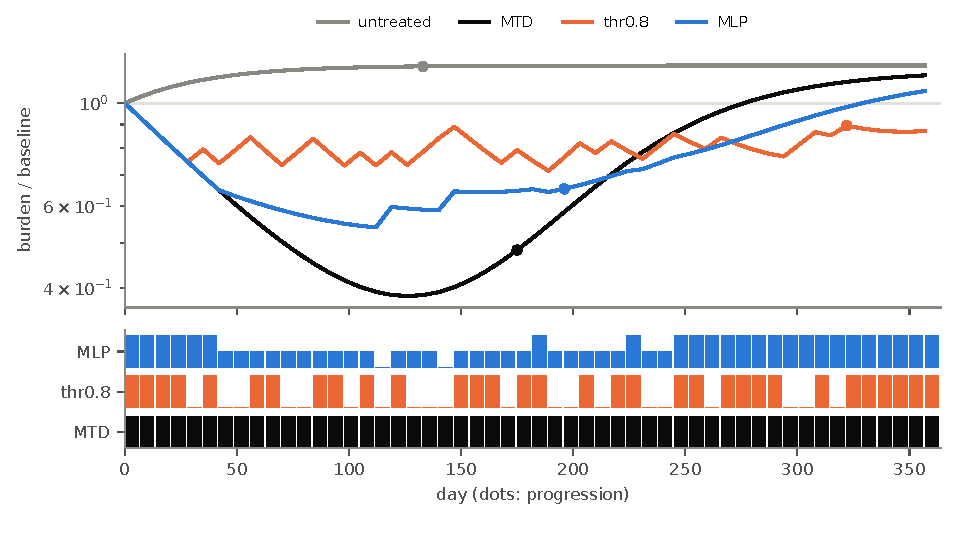
\includegraphics[width=\linewidth]{figures/fig_task.pdf}
\caption{The task. One Tier-1 patient (Strobl ranges) under no treatment, MTD,
thr0.8 and a trained MLP (seed 31, $w=0.1$); dots mark progression. The patient
is the one whose drug saved by the MLP against MTD is the median over the
patients where it saves any, a fixed rule rather than a hand pick. MTD
pushes the burden lowest and progresses at 175\,d; thr0.8 and the MLP
cut the dose, keep the burden nearer baseline, and progress at 322\,d and
196\,d. In this model MTD progresses because the drug acts on $S$ only: once $S$ is cleared, the resistant cells $R$ regrow into the freed capacity (competitive release) and the burden follows them upward although the dose stays maximal. The cut-dose policies keep some $S$ alive to hold $R$ back. Bars show the dose chosen each week.}\label{fig:task}
\end{figure}

\section{Results}\label{sec:results}
Table~\ref{tab:runs} lists every run behind these results, with what it changed and whether it was registered before it ran.
\begin{figure}[t]
\centering
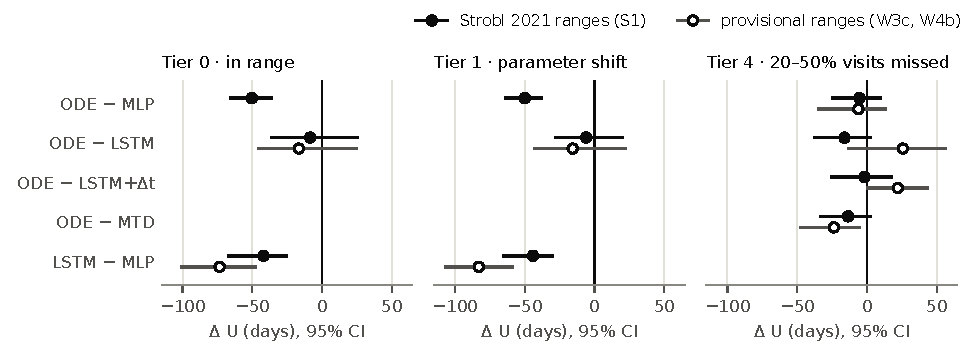
\includegraphics[width=\linewidth]{figures/fig_forest.pdf}
\caption{$\Delta U$ (days) with 95\% CIs over training seeds and patients.
Filled: Strobl ranges (10 seeds per tier and arm). Hollow: provisional
ranges (Tiers 0/1: 5 seeds, per-cell closed-loop gate; Tier 4: 10 seeds,
intention-to-treat). A continuous-time edge needs every ODE row of a
panel right of zero.}
\label{fig:forest}
\end{figure}

\begin{table}[t]
\centering\footnotesize
\caption{All paired differences in one place ($\Delta U$, days, 95\% CI over
training seeds and patients; Strobl ranges, 10 seeds per cell). The ODE-RNN is at
or below its discrete counterparts in every column; a clock or memory costs
tens of days at regular visits. Rows marked $^\dagger$ come from the dropout
experiments (V9, V10).}
\label{tab:summary}
\begin{tabular}{@{}lccc@{}}
\toprule
$\Delta U$ & Tier 0 & Tier 1 & Tier 4 ($p=0.2,0.5$) \\
\midrule
ODE-RNN $-$ MLP & \SAOdeMlpZero & \SAOdeMlpOne & \SBOdeMlp \\
ODE-RNN $-$ LSTM & \SAOdeLstmZero & \SAOdeLstmOne & \SBOdeLstm \\
LSTM $-$ MLP & \SAMemZero & \SAMemOne & --- \\
ODE-RNN $-$ MTD & --- & --- & \SBOdeMtd \\
Positional MLP $-$ MLP & $-53.0$~[$-65.4$, $-40.9$] & $-56.8$~[$-64.2$, $-48.3$] & $+2.2$~[$-13.2$, $+16.4$] \\
Clock-dropout MLP $-$ MLP$^\dagger$ & $-7.5$~[$-10.3$, $-4.5$] & $-2.4$~[$-5.2$, $+0.4$] & --- \\
LSTM, state dropout $-$ LSTM$^\dagger$ & $-2.2$~[$-21.0$, $+17.7$] & $+4.3$~[$-13.1$, $+21.5$] & --- \\
ODE-RNN, state dropout $-$ ODE-RNN$^\dagger$ & $+3.5$~[$-11.6$, $+20.3$] & $+4.2$~[$-8.8$, $+18.9$] & --- \\
\bottomrule
\end{tabular}
\end{table}

\paragraph{Regular visits: memory does not help.} The first question is whether
any recurrent or continuous-time arm beats the MLP when visits are regular. On
Strobl's ranges (Fig.~\ref{fig:forest}) the ODE-RNN scores \SAOdeMlpOne\ against the MLP at
Tier~1 and \SAOdeMlpZero\ at Tier~0, and all ten seeds are negative. Against the
LSTM it scores \SAOdeLstmOne, and the LSTM itself is \SAMemOne\ against the MLP.
Tiers~0 and~1 agree, so the gap is a deficit in control that is already there
without any shift. The provisional regime gives the same ordering (LSTM$-$MLP
\WCMemOne, ODE$-$LSTM \WCOdeLstmOne).

The deficit is not specific to memory. A positional MLP, which is memoryless but
is told the elapsed time, trails the MLP by about as much ($-56.8$ days at
Tier~1, Table~\ref{tab:summary}) and ties the LSTM and the ODE-RNN. Only 0.26 of
its doses are explained by the current observation, against 0.48 for the MLP
and 0.23 for the ODE-RNN. The trainer seems to take a shortcut
(Fig.~\ref{fig:shortcut}): it fits a schedule keyed to the clock instead of
reacting to the tumour. If the clock is hidden in half of the training
episodes, the same network recovers ($+54.4$ [$+44.9$, $+62.3$] over the
positional MLP at Tier~1) and ties the MLP ($-2.4$ days). Scrambling the clock
after training costs only $-14.6$ days, with an interval that spans zero, and
when visits are missed at random the positional MLP ties the MLP ($+2.2$ days).
The same trick does not rescue the recurrent arms. Resetting their memory in
half of the training episodes gains the LSTM and the ODE-RNN about $+4$ days at
Tier~1 (intervals span zero), and both stay 40 to 46 days below the MLP.


\begin{figure}[t]
\centering
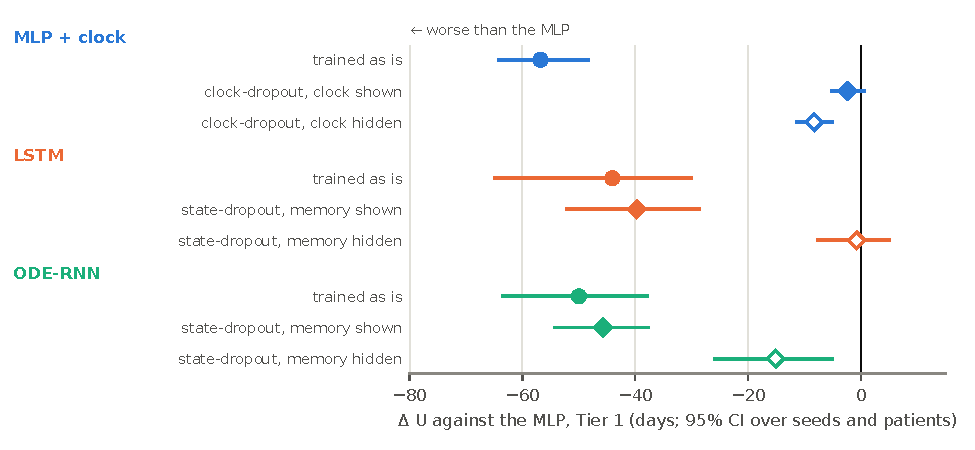
\includegraphics[width=\linewidth]{figures/fig_shortcut.pdf}
\caption{The extra-input deficit is a training shortcut for the clock, not for
memory. $\Delta U$ against the MLP at Tier~1 (Strobl ranges, seeds 31--40).
Circles: trained as is. Filled diamonds: trained with the clock (MLP) or the
recurrent state (LSTM, ODE-RNN) unavailable in half of the episodes, tested with
it available; hollow diamonds: tested with it hidden. Dropout removes the clock's
deficit but not the recurrent ones. Both dropout experiments (V9, V10) were registered before they ran.}
\label{fig:shortcut}
\end{figure}

\begin{figure}[t]
\centering
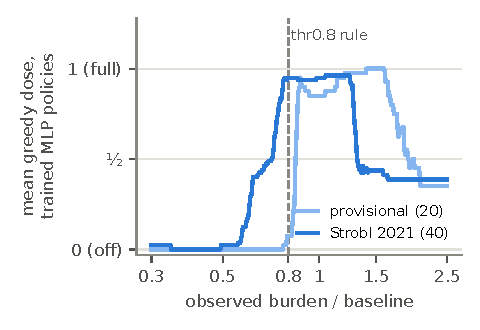
\includegraphics[width=0.5\linewidth]{figures/fig_rule.pdf}
\caption{Mean greedy dose of the trained MLP policies against the observed
burden. The switch-on point sits near the thr0.8 rule. The step down above
${\sim}1.4\times$ baseline (Strobl ranges) lies where 99.9\% of visits are
already past progression, so a dose there only costs exposure.}
\label{fig:rule}
\end{figure}

\paragraph{The best learned policy is a threshold.} Next we ask what the winning
policy actually does. A memoryless MLP's dose is a function of the current observation, so what matters is the shape of that
function (Fig.~\ref{fig:rule}). On Strobl's ranges the mean dose crosses one
half at $\RuleHalfStrobl\times$ baseline and is full by $0.8\times$. A one-line
rule that doses fully above $0.8\times$ baseline (thr0.8) matches it: mean $U$ is
\SAUMlpOne\ for the MLP against \SAUThrOne\ for the rule at Tier~1, and
\SAUMlpZero\ against \SAUThrZero\ at Tier~0. With PQN's published parallelism
(below) the MLP ends slightly above the rule, \SThreeUMlpZero\ against
\SThreeUThrZero\ at Tier~0, by dosing less.

\paragraph{What memory could have bought.} The third question is how much room
the task leaves for memory at all. At regular visits the simulator is
deterministic given the doses, so the best policy with full information is just
the best dose sequence for each patient, and no trainer is needed to bound it. A
search on the true simulator, run per test patient, beats the MLP by $+23.1$
[$+20.3$, $+25.8$] days of $U$. A threshold rule whose level is tuned to each
patient does better still, $+26.0$ [$+23.5$, $+28.5$]: 14 to 19 more days to
progression on 46 to 60 fewer days of drug. The task therefore has room that the
MLP does not reach.

That room splits into three near-equal parts (Table~\ref{tab:split}). About a
third is a fixed memoryless threshold near baseline, which the MLP could
represent but did not learn, because its training reward charges for burden
between the nadir line and baseline. Another third comes from seeing the burden
exactly instead of with 5\% noise, which bounds what filtering the observation
history could recover. The last third comes from knowing each patient's best
level, which bounds what inferring the patient from history could add. For a
threshold policy, then, information that memory could supply is worth at most
about 15 days, while the learning cost of the recurrent arms was 40 to 50. This is a
split of one rule family's gain and not a bound on memory: the per-patient
search ($+23.1$) is itself below the tuned threshold ($+26.0$), so it is not the
full-information optimum, and the first two rows of the table are post hoc.
Read together with the trainer results below, the negative result is about
PQN at this budget. It is a learning cost larger than the benefit we can
measure, which is not a proof that memory has none.

The recurrent arms also reach a lower training reward than the MLP on their own
training patients ($-20.7$ and $-23.5$ reward units, intervals exclude zero), so
they optimise the reward less well.
A reference network trained like the arms but also shown $S$, $R$ and $\theta$
never reached the headroom. It scored \HFullZero\ below the MLP, then
\SThreeFull\ with PQN's published parallelism, and \TOneFull\ with ten times
the gradient steps, where it ties the MLP on training reward. That reward has no
progression term. Adding one (a survival term paid until progression is
confirmed) lifts the reference by $+15.4$ [$+10.2$, $+20.8$] days and brings it
level with the MLP ($-1.4$ [$-4.1$, $+1.2$]). It now wins on 62 to 69\% of
patients (median $+2$ to $+15$ days, mostly through less drug), but its mean is
lower because of a tail of earlier progressions, so on the mean it recovers none
of the $+23$ days. The reward was part of the gap, and the rest is PQN's
difficulty in using the true state.

\paragraph{Other trainers: none passes our admission rule.} The obvious
objection is that the deficit belongs to PQN. Our own rule for admitting a new
trainer is that a policy shown the true hidden state must beat the burden-only
MLP under it. We tried two. PPO (600 updates, untuned, all arms retrained) fails
the rule ($-1.6$ [$-10.4$, $+5.6$] at Tier~0). So does recurrent Q-learning
with an episode replay buffer, a target network and $n$-step double-Q targets,
the recipe of R2D2 \cite{kapturowski2019} applied to whole episodes
($-3.9$ [$-8.3$, $+0.9$] at Tier~0, $-1.8$ [$-6.0$, $+2.2$] at Tier~1; the
recurrent arms were not run). The reference does have a smaller burden
integral at the same median dose, which suggests that the capped-TTP score
under-credits it. Neither run can say whether the deficit belongs to PQN, and
we do not claim it holds under three trainers. Descriptively under PPO, the
LSTM and ODE-RNN again trail the MLP ($-40.7$ and $-42.3$ days at Tier~1, and
they tie each other), and in 12 and 22 of 40 cells they collapse to a fixed
full-dose schedule, the failure described in \S\ref{sec:pitfalls}, item~1. We
still lack a trainer under which the reference beats the MLP.


\paragraph{Is the LSTM too small?} No evidence for it. An LSTM with 64 or 128
units (5 and 22 times the parameters) scores $-5.1$ [$-26.8$, $+18.6$] and
$-3.1$ [$-25.0$, $+26.2$] days against the 26-unit one at Tier~1, and stays $-49$
and $-47$ days below the MLP. The intervals are wide, so the registered reading
is ``inconclusive'' against our 10-day gate, but neither size recovers anything.
We did not scale the MLP or the ODE-RNN.

\paragraph{Representation or learning?} We behaviour-cloned a threshold teacher
(a fixed level, or a level tuned to each patient) into each arm. For the fixed
threshold every arm reaches the teacher's score: the cloned MLP, LSTM and
ODE-RNN get $U=284.6$, 284.7 and 284.6, so the recurrent networks can represent
a good policy. Cloning the patient-tuned level, which a burden-only student can
recover only from history, shows no memory gain (LSTM $-2.5$ [$-10.6$, $+6.5$];
ODE-RNN $+1.8$ [$-9.9$, $+13.1$], inconclusive against the 10-day gate). We then
fine-tuned the cloned fixed-threshold policies with PQN. The MLP stays where it
was ($-0.5$ [$-5.1$, $+4.6$]), while the LSTM loses $-69.0$ [$-92.3$, $-48.1$]
days and the ODE-RNN $-87.7$ [$-121.1$, $-60.2$], with 2 to 12\% of recurrent
cells collapsing to open loop. So the recurrent deficit is a cost of training
them with PQN, not a limit on what they can represent. It does not show that
another trainer would avoid the cost, and the two trainers above cannot either.


\paragraph{Can this trainer use memory at all?} Yes, where memory pays. On
three POPGym tasks \cite{morad2023}, run in the JAX port of \citet{lu2023}, the
same PQN update trains an LSTM that beats a parameter-matched MLP on two (return,
with perfect $=+1$: RepeatPrevious $+1.38$ [$+1.23$, $+1.49$], RepeatFirst
$+1.04$ [$+0.67$, $+1.39$], 10 seeds). On the third, CountRecall, neither arm
learns ($+0.04$). The LSTM is unstable across seeds here as on the cancer task:
4 of 10 RepeatFirst seeds end below $+0.1$. So the recurrent deficit is not a
trainer that cannot represent memory. It is specific to this task and signal.
These are two easy tasks, one trainer and no tuning.

\begin{table}[t]
\centering\footnotesize
\caption{Where the full-information headroom comes from (Tier~0, days of $U$,
mean over the four exposure prices, CIs over seeds and patients). Rows 1 and 2
are post hoc. Fixed levels are chosen on the other nine seeds' patients.}
\label{tab:split}
\begin{tabular}{@{}lll@{}}
\toprule
Component & $\Delta U$ & Needs \\
\midrule
Best fixed threshold under noise ($\approx 1.0\times$) $-$ MLP & $+10.8$ [$+8.1$, $+13.3$] & nothing the MLP lacks \\
Exact vs noisy observation, fixed threshold & $+8.6$ [$+7.2$, $+10.5$] & filtering (memory) \\
Patient-tuned vs fixed threshold & $+6.6$ [$+6.0$, $+7.2$] & inferring the patient (memory) \\
\midrule
Patient-tuned threshold $-$ MLP (total) & $+26.0$ [$+23.5$, $+28.5$] & \\
\bottomrule
\end{tabular}
\end{table}

\begin{figure}[t]
\centering
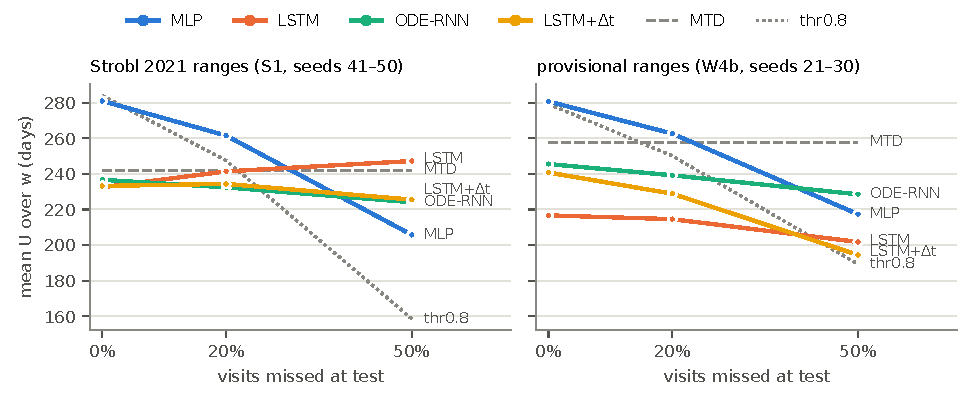
\includegraphics[width=\linewidth]{figures/fig_missed.pdf}
\caption{Mean $U$ over the four exposure prices against the share of visits
missed at test. All arms were trained with 35\% of visits missed; 10 seeds per
arm. Grey: MTD (dashed) and the thr0.8 rule (dotted).}
\label{fig:missed}
\end{figure}

\paragraph{Missed visits: no continuous-time edge.} Missed visits are where a
continuous-time state should help most, so we ask whether it does. Trained with
35\% of visits missed, the ODE-RNN is above none of its comparators on Strobl's ranges
(Fig.~\ref{fig:forest}): against the MLP \SBOdeMlp, against the LSTM
\SBOdeLstm, against LSTM+$\Delta t$ \SBOdeLstmDt, and against MTD \SBOdeMtd. It
degrades more gracefully than the MLP as visits go missing (\SBGraceMlp\ on
$U(p)-U(0)$) but less than the LSTM (\SBGraceLstm), so graceful degradation
comes from recurrence and not from continuous time. The ODE-RNN's one advantage
over the MLP, at $p=0.5$, is an exposure artefact: it doses more (median
exposure 326 against 194 at $w=0.1$), and the comparison already nets that drug
out in $U$.
The provisional regime agrees (ODE$-$MLP \WBOdeMlp, ODE$-$MTD \WBOdeMtd). One
Tier~4 effect is unstable: adding $\Delta t$ to the LSTM changed $U$ by $+38.8$,
$+3.5$ and $-14.4$ in three independent runs, so we read differences involving
LSTM+$\Delta t$ as seed noise.

\paragraph{Missed visits remove the value of feedback.} The MLP, which is best at
regular visits, loses the most as visits go missing (Fig.~\ref{fig:missed};
mean $U$ goes from \SBUMlpZero\ to \SBUMlpHalf\ on Strobl's ranges, and for
thr0.8 from \SBUThrZero\ to \SBUThrHalf). When a visit is missed the last dose
continues, so a threshold policy that has switched off keeps the drug off
through the gap while the tumour regrows. At 20\% missed the MLP is still above
MTD (\SBUMlpFifth\ against \SBUMtdFifth). At 50\% no learned policy is above MTD
in either regime over our one-year horizon (but see \S\ref{sec:monitoring} for
three years). On Strobl's ranges the best arm, the LSTM, ties it (\SBFb); the
MLP (\SBFbMlp) and LSTM+$\Delta t$ (\SBFbLstmDt) are below it, and the ODE-RNN is
at or below it (\SBFbOde). On the provisional ranges all four arms are below it
(best: \WBFbBest, \WBFb).

These statements are about the mean. For the median patient the LSTM beats MTD
($+10.7$ [$+1.7$, $+28.0$]): about 45\% of patients are progression-free under
both at one year, and the LSTM uses less drug on them. Replayed unchanged over
three years, every learned arm beats MTD on $U$ by 32 to 82 days, but only the
LSTM matches its time to progression ($+9.0$ [$-9.4$, $+28.6$] days). The others
progress earlier and win on drug saved, as the threshold rules do
(\S\ref{sec:monitoring}). The ODE-RNN shows no edge there either (ODE$-$LSTM
$-32.1$ [$-70.9$, $+9.1$]).

\paragraph{Models fitted to patients; monitoring maps.} Replaying the saved
policies on models fitted to 55 prostate-cancer patients, both negatives
replicate (Appendix~\ref{sec:fitted}). Whether feedback survives missed visits
need not depend on architecture at all: with threshold rules only, it stops
beating MTD at 10--50\% missed visits over one year, and the crossover depends
on cost of resistance, turnover and horizon (Appendix~\ref{sec:monitoring}).

\section{Four evaluation errors}\label{sec:pitfalls}
Early in the project we made four mistakes that each produced a result that
looked publishable. We list them because the controls that found them are cheap
and apply to similar claims.
\begin{enumerate}
\item The first was open-loop collapse. Under PPO the ODE-RNN gave all 200
patients one identical exposure in 4 of 6 cells, so our first ``architecture''
result compared feedback with a fixed schedule. The cause was initialisation:
each 7-day flow drove the hidden state to a saturated fixed point, and an
untrained policy's entropy fell from 1.07 to 0 within one episode.

\item The second was a validity gate that became wrong under missed visits. Once
observations were unreliable, near-fixed schedules scored higher than
closed-loop cells, so excluding them biased the comparison. We moved to
intention-to-treat and added MTD as a reference arm to beat.
\item The third was training instability that looked like an architecture effect.
A change of $2\times10^{-7}$ in a float moved one ODE-RNN cell's mean $U$ from
132 to 256 days. Intervals over patients alone ($[-20,-11]$) showed the ODE-RNN
worse than the LSTM, and resampling training seeds widened them to $[-43,+22]$.

\item The fourth was a mis-built shifted cohort. Shifting $K$ after computing
$y_0$ put 43 to 50\% of Tier-1 patients above capacity. Under full dose 14 to
18\% of them diverged to NaN, and these were scored as censored, that is, as
successes. A progressor-only TTP median and TTP bought with extra drug misled us
in similar ways, which is why every comparison here uses the censoring-aware
estimator and the exposure term.
\end{enumerate}

\begin{table}[t]
\centering\footnotesize
\caption{Controls for claims about memory or continuous time in partially
observed RL: what each catches here, and its cost.}
\label{tab:controls}
\resizebox{\linewidth}{!}{\begin{tabular}{@{}p{0.34\linewidth}p{0.40\linewidth}p{0.22\linewidth}@{}}
\toprule
Control & Error it catches here & Cost \\
\midrule
Memoryless and clock-only baselines & ``Memory helps'' when a threshold does as well; a clock costs as much as memory (V7) & two extra arms \\
Trainer-free headroom bound, split by information & ``Undertrained recurrent nets'': memory could buy $\le 15$\,d (O1b) & one search on the simulator \\
CIs over training seeds and test cases & A patient-only CI that held trained policies fixed (item 3) & $\ge 5$ seeds per arm \\
Policy cost next to its score & TTP bought with drug; progressor-only medians (item 4) & one exposure term \\
Failed runs kept in the count & A validity gate that selected the better cells (item 2); open-loop collapse (item 1) & intention-to-treat reporting \\
\bottomrule
\end{tabular}}
\end{table}



\section{Limitations}\label{sec:limits}
The study uses one ODE family, Lotka--Volterra with competition between
sensitive and resistant cells, and virtual patients only. It makes no claim
about clinical outcomes.

\paragraph{The trainer.} PQN's settings are the published ones, untuned, except
for parallelism (32 patients per update, not 1024). The recurrent arms are
unstable in training, and we count that as part of their cost instead of tuning
it away. The warm-start experiment supports reading the deficit as a learning
cost of PQN (\S\ref{sec:results}), but it uses PQN throughout, so it cannot say
whether another trainer avoids the cost. Given the true hidden state, PQN at the
registered budgets scores below the burden-only MLP. With ten times the
gradient steps it matches the MLP on training reward and still trails on $U$,
and with a progression term in the reward it ties the MLP on mean $U$. Neither
change opened the registered 10-day gate, so we stopped the reward and budget
search there instead of tuning until it passed.

\paragraph{The architectures.} We test one continuous-time design, the ODE-RNN;
liquid time-constant networks \cite{hasani2021} and neural CDEs
\cite{kidger2020} are untested. Missed visits are i.i.d., so the next gap is
unknown when the policy doses and carries no information. On a fixed visit
schedule with the time to the next visit given as an input, the ODE-RNN is below
the MLP on held-out schedules ($-21.4$ [$-42.8$, $-2.9$]). Trained on a pool of
schedules it is above the MLP ($+34.8$ [$+16.1$, $+53.7$]), but so is the LSTM,
and the MLP never gains from the input ($+1.4$ [$-10.3$, $+14.4$]), so neither
run tests whether a known schedule helps a continuous-time state.


\paragraph{The simulator.} Before testing mechanism shift (Tier~2) we checked
four other tumour models. Kuznetsov has no resistant population, so MTD is
optimal by construction. Hahnfeldt is a mouse model with no resistant
population, and our implementation reproduces it in its own units except for
two narrow misses \cite{hahnfeldt1999}. The three-population model behind the
clinical adaptive-therapy trial \cite{zhang2017} reproduces structurally (22 of
22 equilibria) but not in its published progression times (at most 15 of 40).

A tumour--immune model in which chemotherapy also kills immune cells
\cite{depillis2006} reproduces its source's qualitative outcomes but leaves no
room for a dosing comparison: a rule tuned to each patient beats MTD by only 1.7
days [1.0, 3.0], against our gate of 10, because outcomes are set by the
patient's immune state and not by the dosing.
LV is therefore the only family here with a resistance mechanism, and every
result is LV-only. Within LV the negatives hold on two parameter regimes, under
a parameter shift, and on models fitted to 55 patients, and our implementation
reproduces Strobl et al.'s published times to progression. Within-episode drift
(Tier~3) is untested.

\paragraph{Horizon and metrics.} The learned policies were compared over one
year only. The monitoring maps show that the value of feedback under missed
visits depends on the horizon, so ``no learned policy beats MTD at 50\% missed''
is a one-year statement about the mean. The maps cover threshold rules only, and
over one year at low turnover the best rule sits at the grid's most aggressive
level. $U$ is a mean. On medians the three-year win holds only where resistance
is nearly free, and the sparing rules always carry a larger tumour burden, which
our metastasis proxy counts against them.

\section{Conclusion}\label{sec:conclusion}
On this task a memoryless burden threshold is a strong baseline, and neither
memory nor continuous time beat it, on two parameter regimes and on models
fitted to 55 patients' PSA. The task does have headroom, but the part that memory could supply is at most
about 15 days, smaller than the learning cost of the recurrent arms (40 to 50
days), and the warm-start experiment points to PQN's training and not to a limit
on what the networks can represent. Even given the hidden state, and with a
reward that pays until progression, the same trainer only ties the burden-only
MLP. When half of the visits are missed, the question changes from which
architecture uses feedback best to whether feedback has any value, and over one
year, on average, it had none. We think a fair test of a continuous-time policy needs a
setting where the gap itself carries information, such as scheduled instead of
random visits, and a trainer that can first beat the threshold with the true
state.

\paragraph{Broader impact.} All patients are simulated; the paper makes no clinical claim and no policy here is a treatment recommendation. We see no significant risk of harm.

\paragraph{Controls for similar claims.} Before reporting an architecture
effect in partially observed RL, we suggest the five controls of
Table~\ref{tab:controls}.

\begin{thebibliography}{99}
\bibitem[Gallagher et~al.(2024)Gallagher, Strobl, Park, Spoendlin, Gatenby, Maini, and Anderson]{gallagher2024} K.~Gallagher, M.~A.~R. Strobl, D.~S. Park,
F.~C. Spoendlin, R.~A. Gatenby, P.~K. Maini, A.~R.~A. Anderson. Mathematical
model-driven deep learning enables personalized adaptive therapy. \emph{Cancer
Research} 84(11):1929--1941, 2024. \url{https://doi.org/10.1158/0008-5472.CAN-23-2040}.
\bibitem[Strobl et~al.(2021)Strobl, West, Viossat, Damaghi, Robertson-Tessi, Brown, Gatenby, Maini, and Anderson]{strobl2021} M.~A.~R. Strobl, J.~West, Y.~Viossat, M.~Damaghi,
M.~Robertson-Tessi, J.~S. Brown, R.~A. Gatenby, P.~K. Maini, A.~R.~A. Anderson.
Turnover modulates the need for a cost of resistance in adaptive therapy.
\emph{Cancer Research} 81(4):1135--1147, 2021. \url{https://doi.org/10.1158/0008-5472.CAN-20-0806}.
\bibitem[Kiram et~al.(2026)Kiram, Youkana, Saouli, Susto, and Kahloul]{kiram2026} F.~M.~E. Kiram, I.~Youkana, R.~Saouli, G.~A. Susto,
L.~Kahloul. Recurrent deep reinforcement learning for chemotherapy control
under partial observability. \url{https://arxiv.org/abs/2605.02552}, 2026.
\bibitem[Hahnfeldt et~al.(1999)Hahnfeldt, Panigrahy, Folkman, and Hlatky]{hahnfeldt1999} P.~Hahnfeldt, D.~Panigrahy, J.~Folkman, L.~Hlatky.
Tumor development under angiogenic signaling: a dynamical theory of tumor
growth, treatment response, and postvascular dormancy. \emph{Cancer Research}
59(19):4770--4775, 1999. PMID 10519381, \url{https://pubmed.ncbi.nlm.nih.gov/10519381/}.
\bibitem[Zhang et~al.(2017)Zhang, Cunningham, Brown, and Gatenby]{zhang2017} J.~Zhang, J.~J. Cunningham, J.~S. Brown, R.~A. Gatenby.
Integrating evolutionary dynamics into treatment of metastatic
castrate-resistant prostate cancer. \emph{Nature Communications} 8:1816, 2017.
\url{https://doi.org/10.1038/s41467-017-01968-5}.
\bibitem[Rubanova et~al.(2019)Rubanova, Chen, and Duvenaud]{rubanova2019} Y.~Rubanova, R.~T.~Q. Chen, D.~Duvenaud. Latent ODEs
for irregularly-sampled time series. \emph{NeurIPS}, 2019. \url{https://arxiv.org/abs/1907.03907}.
\bibitem[Gallici et~al.(2024)Gallici, Fellows, Ellis, Pou, Masmitja, Foerster, and Martin]{gallici2024} M.~Gallici, M.~Fellows, B.~Ellis, B.~Pou, I.~Masmitja,
J.~N. Foerster, M.~Martin. Simplifying deep temporal difference learning.
\url{https://arxiv.org/abs/2407.04811}, 2024.
\bibitem[Kidane et~al.(2026)Kidane, Motayed, and Wang]{kidane2026} B.~S. Kidane, M.~S.~H. Motayed, S.~Wang. Adaptive
chemotherapy control under tumor heterogeneity via reinforcement learning.
\url{https://arxiv.org/abs/2609.12264}, 2026.
\bibitem[Ni et~al.(2022)Ni, Eysenbach, and Salakhutdinov]{ni2022} T.~Ni, B.~Eysenbach, R.~Salakhutdinov. Recurrent model-free RL
can be a strong baseline for many POMDPs. \emph{ICML}, PMLR 162, 2022. \url{https://arxiv.org/abs/2110.05038}.
\bibitem[Morad et~al.(2023)Morad, Kortvelesy, Bettini, Liwicki, and Prorok]{morad2023} S.~Morad, R.~Kortvelesy, M.~Bettini, S.~Liwicki,
A.~Prorok. POPGym: benchmarking partially observable reinforcement learning.
\emph{ICLR}, 2023. \url{https://arxiv.org/abs/2303.01859}.
\bibitem[Lu et~al.(2023)Lu, Schroecker, Gu, Parisotto, Foerster, Singh, and Behbahani]{lu2023} C.~Lu, Y.~Schroecker, A.~Gu, E.~Parisotto, J.~Foerster, S.~Singh, F.~Behbahani. Structured state space models for in-context reinforcement learning. \emph{NeurIPS}, 2023 (\url{https://arxiv.org/abs/2303.03982}); we use only its JAX re-implementation of POPGym, github.com/luchris429/popjaxrl.
\bibitem[Kidger et~al.(2020)Kidger, Morrill, Foster, and Lyons]{kidger2020} P.~Kidger, J.~Morrill, J.~Foster, T.~Lyons. Neural
controlled differential equations for irregular time series. \emph{NeurIPS},
2020. \url{https://arxiv.org/abs/2005.08926}.
\bibitem[Hasani et~al.(2021)Hasani, Lechner, Amini, Rus, and Grosu]{hasani2021} R.~Hasani, M.~Lechner, A.~Amini, D.~Rus, R.~Grosu. Liquid
time-constant networks. \emph{AAAI} 35(9), 2021. \url{https://arxiv.org/abs/2006.04439}.
\bibitem[de Pillis et~al.(2006)de Pillis, Gu, and Radunskaya]{depillis2006} L.~G. de Pillis, W.~Gu, A.~E. Radunskaya. Mixed immunotherapy and
chemotherapy of tumors: modeling, applications and biological interpretations. \emph{J. Theor. Biol.} 238(4):841--862, 2006. \url{https://doi.org/10.1016/j.jtbi.2005.06.037}.
\bibitem[Lu et~al.(2024)Lu, Chu, Li, Wang, Gatenby, and Zhang]{lu2024} Y.~Lu, Q.~Chu, Z.~Li, M.~Wang, R.~Gatenby, Q.~Zhang. Deep reinforcement
learning identifies personalized intermittent androgen deprivation therapy for prostate cancer. \emph{Briefings in Bioinformatics} 25(2):bbae071, 2024.
\url{https://doi.org/10.1093/bib/bbae071}.
\bibitem[Kuosmanen et~al.(2021)Kuosmanen, Cairns, Noble, Beerenwinkel, Mononen, and Mustonen]{kuosmanen2021} T.~Kuosmanen, J.~Cairns, R.~Noble, N.~Beerenwinkel, T.~Mononen, V.~Mustonen.
Drug-induced resistance evolution necessitates less aggressive treatment. \emph{PLoS Computational Biology} 17(9):e1009418, 2021.
\url{https://doi.org/10.1371/journal.pcbi.1009418}.
\bibitem[Kapturowski et~al.(2019)Kapturowski, Ostrovski, Quan, Munos, and Dabney]{kapturowski2019} S.~Kapturowski, G.~Ostrovski, J.~Quan, R.~Munos, W.~Dabney.
Recurrent experience replay in distributed reinforcement learning. \emph{ICLR},
2019. \url{https://openreview.net/forum?id=r1lyTjAqYX}.
\end{thebibliography}

\appendix
\begin{figure}[t]
\centering
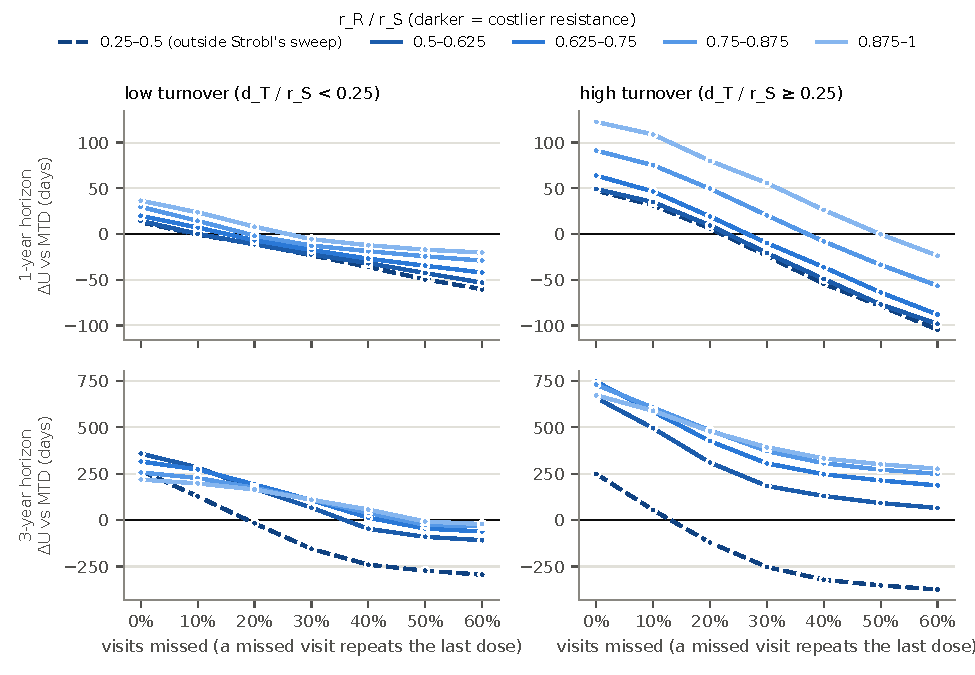
\includegraphics[width=\linewidth]{figures/fig_monitoring.pdf}
\caption{Where monitoring stops being useful. The best threshold rule minus MTD in
$U$ (mean over the four exposure prices) on held-out test patients, against the
share of visits missed. The threshold is chosen on a separate selection cohort.
Lines are bins of $r_R/r_S$; darker means a costlier resistance, and the dashed
bin lies outside Strobl et al.'s sweep. A missed visit repeats the last dose.
Rows: the same patients followed for one year (top) and three years (bottom);
note the different $y$-scales. 10 seeds $\times$ 200 test patients per bin.
Registered: one year (M1) and three years (M1b). The median analysis in the
text (M1c) is post hoc.}
\label{fig:monitoring}
\end{figure}

\section{Models fitted to patients}\label{sec:fitted}
Strobl et al.\ fitted this model to
PSA from \RTwoN\ men in an intermittent androgen-suppression trial
\cite{strobl2021}. We repeated their fit with our simulator: \RTwoExcl\ fits
fail their $r^2 \ge 0.5$ rule (theirs: 15), and fitted cost and turnover are
anticorrelated (\RTwoPearson; theirs $-0.77$). Their relapse separation holds in
direction only ($p = \RTwoMWp$, post hoc after a mis-registered test). Replaying
the saved policies, unchanged, on the \POneN\ kept fits: at regular visits
ODE-RNN$-$MLP is \POneOdeMlp\ and ODE-RNN$-$LSTM \POneOdeLstm; with half the
visits missed, no learned arm beats MTD (ODE-RNN \POneOdeMtd, LSTM
\POneLstmMtd). MTD keeps every fitted patient progression-free for a year, so
this replay tests drug use more than progression time. These are models fitted
to patients, not patients.

\section{When does monitoring stop being useful?}\label{sec:monitoring}
Whether feedback survives missed visits need not depend on architecture at all.
We binned patients by cost of resistance ($r_R/r_S$) and turnover ($d_T/r_S$).
In each bin we compared the best burden-threshold rule with MTD, with rules
only and no learning (Fig.~\ref{fig:monitoring}; pre-registered). The rule's
level is chosen on a selection cohort and scored on test patients. With
reliable monitoring, feedback beats MTD in every bin, by \MOneRegMin\ to
\MOneRegMax\ days over one year. The share of missed visits at which it stops
doing so rises as resistance becomes cheaper: from \MOnePStarLowMin\ to
\MOnePStarLowMax\ at low turnover, and from \MOnePStarHighMin\ to
\MOnePStarHighMax\ at high turnover. At 50\% missed, the costliest bin inside
Strobl's sweep trails the no-cost end by \MOneCostLow\ days at low turnover
and \MOneCostHigh\ at high turnover. Feedback thus tolerates unreliable
monitoring best where adaptive therapy helps most \cite{strobl2021}.

\paragraph{The horizon changes the answer.} Over one year, MTD reaches the end of
the horizon for most patients in the costliest bins, so we followed the same
patients for three years (Fig.~\ref{fig:monitoring}, bottom). The cost effect
survives: \MOneBCostLow\ and \MOneBCostHigh\ days at 50\% missed. The crossover
moves later, to \MOneBPStarLowMin--\MOneBPStarLowMax\ at low turnover and
\MOneBPStarHigh\ at high turnover. There, sparing thresholds beat MTD by
\MOneBHighMin\ to \MOneBHighMax\ days at 50\% missed. Within three years MTD
fails in nearly every patient inside Strobl's range, while sparing dosing holds
a minority for the whole horizon. At the no-cost end, \MOneBTailCens\ of
patients never progress under the threshold rule, which uses \MOneBExpCut\ less
drug. Its \emph{median} TTP is nonetheless shorter than MTD's (\MOneBMedThr\ vs
\MOneBMedMtd\ days): the gain is a heavy right tail plus drug saved, which $U$
rewards and the median does not. Dosing through missed visits, which helped
over one year (\MOneMiss), now helps at low turnover but hurts at high turnover
(pooled \MOneBMiss).

\paragraph{Medians narrow the claim.} $U$ above is a mean over patients. Scored
on medians instead (a post-hoc analysis of the same runs, with the threshold
also chosen by median), the three-year gain at high turnover and 50\% missed
survives only in the two lowest-cost bins, $\hat r_R \ge 0.75$ (\MOneCHighThree\
and \MOneCHighFour\ days). In the two costliest bins inside Strobl's sweep it
reverses (\MOneCHighOne\ and \MOneCHighTwo). The cost effect holds under medians
over three years but not over one year at low turnover (\MOneCCostOneLow). In
all 20 bin$\times$horizon cells at 50\% missed, the selected threshold rule has
a shorter median TTP and a larger median burden integral than MTD (by
\MOneCBurdenNoCost\ at the three-year no-cost end, $\MOneCBurdenCostly\times$ in
the costliest Strobl bin). Where sparing wins for the median patient, it wins
on drug saved, not on time bought or tumour held down.


\section{Simulator and protocol in detail}\label{sec:methods}
This appendix states every modelling and protocol choice behind the results, so
that the experiments can be read without the code.

\paragraph{Tumour model.} State $(S,R)$: sensitive and resistant cells,
in the equations of \S\ref{sec:setup}. Both populations grow logistically toward the shared
capacity; the drug acts on the sensitive growth term only, through
$(1-d_D u)$, and both populations die at their own rates $d_S, d_R$. The
resistant population pays a cost of resistance ($r_R<r_S$) and is untouched by
the drug, so continued full dosing selects for it, which is what adaptive
therapy tries to avoid. The primary parameter ranges are those of Strobl et al.\
(2021); a patient is one Latin-hypercube draw of $(r_R/r_S,\,d_T/r_S,\,n_0,\,f_R)$
with $r_S$, $d_D$ fixed. A second, stronger-cost regime is reported separately.

\paragraph{Drug.} A dose is a bolus added to a single compartment, cleared
exponentially at $0.5\,\mathrm{d}^{-1}$ (closed form between visits). The
treatment intensity is $u = C/(C+EC_{50})$ with $EC_{50}=0.5$, so doubling a dose
does not double cell kill. The three doses are $\{0,\tfrac12,1\}$.

\paragraph{Time.} One episode is one year: 52 weekly visits, i.e.\ 357\,d.
At every visit the policy sees one observation and chooses a dose; the chosen
dose is administered at the visit and the tumour ODE is then integrated for
7\,d with a fixed-step Tsitouras 5(4) solver (accurate to about $10^{-4}$). An episode always runs the full 52
visits; progression is read off the burden curve afterwards. The ODE-RNN
advances its latent state through each 7-day gap in 8 steps of $7/8$\,d; the MLP
and LSTM treat one visit as one step. At Tier~4 a missed visit produces no
observation and no decision, the previous dose continues, and the
discrete-time arms receive no information about the gap except the LSTM+$\Delta t$
arm.

\paragraph{Observation.} The policy sees one number per visit,
$\log(\text{burden}/\text{baseline})$, where burden is $S+R$ times a log-normal
noise factor with 5\% standard deviation of the log and baseline is the same
patient's burden at visit 0. It never sees $S$, $R$, $\theta$ or the visit index
(except the positional MLP, which sees elapsed time).

\paragraph{Reward and score.} The training reward at a visit is
$-\max(b/b_{\min}-1.2,\,0) - w\cdot\text{dose}$ plus a constant, where $b_{\min}$
is the lowest burden so far; the 1.2 matches the progression definition. One
network is trained per exposure price $w\in\{0.05,0.1,0.2,0.4\}$ and seed.
The reported score $U=\min(\mathrm{TTP},357)-w\cdot\text{exposure}$ uses the same $w$.
Exposure is the cumulative dose over the episode. TTP is the first time the burden has
stayed 20\% above its running nadir for 28 consecutive days (censored at 357\,d
if it never does).

\paragraph{Cohorts and seeds.} For each seed, 200 training patients are drawn
and 200 held-out test patients from the same ranges (Tier~0). Tier~1 rescales
$r_S, r_R$ by 1.5 and $K$ by 0.6 and recomputes the initial state so that no
patient starts above capacity (an earlier build did not; \S\ref{sec:pitfalls}).
Each (arm, $w$, seed) cell is trained from scratch on that seed's training
cohort and then scored greedily on its test cohort. The primary regime uses 10
seeds per arm; the provisional regime uses 5.

\paragraph{Training.} Every arm is trained by PQN with the settings of
Table~\ref{tab:hparams}: 300 updates, each collecting 32 training patients'
full episodes with $\varepsilon$-greedy exploration, followed by 4 epochs of
4 minibatches of whole patient episodes (never shuffled transitions, because a
recurrent Q-value depends on the visits before it). Learning rate, discount and
$\lambda$ are the published values and are the same for every architecture.
No arm is tuned.

\paragraph{Comparisons.} For two arms $A,B$ the paired difference is
$U_A-U_B$ per test patient, averaged over $w$ (and over missed-visit rates at
Tier~4), and the 95\% interval is the 2.5th and 97.5th percentiles of 2000
bootstrap means that resample training seeds and patients. The
registered gates and readings (``edge'', ``deficit'', ``ties'') and every run's
pass and kill criteria were written before the run (Table~\ref{tab:runs}).

\paragraph{What the simulator cannot show.} One resistance mechanism
(competition), parameters from published ranges and not individual patients,
one drug, weekly observations of total burden only, and a one-year horizon in
the primary results. Section~\ref{sec:limits} states the consequences.

\section{Reproducibility}\label{sec:repro}
\begin{table}[h]
\centering\footnotesize
\caption{Settings shared by every arm. PQN values are the published recurrent
settings \cite{gallici2024}, untuned, except parallelism.}
\label{tab:hparams}
\begin{tabular}{@{}ll@{}}
\toprule
Trainer & PQN, Peng's Q($\lambda$), no replay, no target network \\
Learning rate & $3\times10^{-4}$, linear decay to 0 \\
$\gamma$, $\lambda$ & 0.99, 0.5 \\
Epochs $\times$ minibatches & $4\times4$, minibatches of whole patient episodes \\
$\varepsilon$-greedy & $1.0\to0.005$ over the first 10\% of updates \\
Max gradient norm & 0.5 \\
Budget & 300 updates $\times$ 32 patients $\times$ 52 visits (S3: 1024 patients) \\
Reward scale & 0.01 \\
\midrule
MLP & one hidden layer, width 441, LayerNorm \\
LSTM, LSTM+$\Delta t$ & 26 units, LayerNorm Q-readout ($\Delta t$ in units of 7\,d) \\
ODE-RNN & GRU jump, 16-d latent, field width 64, fixed $7/8$\,d steps \\
\midrule
PK & bolus, clearance $0.5\,\mathrm{d}^{-1}$, $E_{\max}$ effect, $EC_{50}=0.5$ \\
Cohorts & 200 training, 200 test patients (Latin hypercube) \\
Seeds & 10 per arm and tier (primary regime); 5 (provisional, Tiers 0/1) \\
\bottomrule
\end{tabular}
\end{table}
Everything is written in JAX, Equinox and Diffrax and runs on CPU (one Intel
i7-13800H); rollouts use fixed-step solvers, which we found accurate to
${\sim}10^{-4}$ and faster than adaptive stepping or GPU at this batch size.
The largest single run (V2, 80 cells at 1024 patients and 3000 updates) took
about 150 CPU-hours. Code, pre-registrations and the dated research log
referenced in Table~\ref{tab:runs} will be released with the paper.

\section{Registered runs}
Run names and log lines refer to the dated, append-only research log released
with the code; each run's hypothesis and pass/kill criteria were registered
before it ran.

\begin{table}[h]
\centering\footnotesize\setlength{\tabcolsep}{4pt}
\caption{Every registered policy comparison, in order, including void and
invalid ones. ``Valid'' means both arms passed the validity rule registered
for that run. ``Reg.'': yes = registered before it ran; post hoc = chosen after
earlier results (O1b only partly). Run names used in the text index this table.}
\label{tab:runs}
\resizebox{\linewidth}{!}{\begin{tabular}{@{}lllll@{}}
\toprule
Run & Change & Outcome & Reg. & Log entry \\
\midrule
Phase 2 & MLP vs ODE-RNN, PPO, Tier 1 & void: cohort above capacity & yes & L242 \\
Phase 2 rerun & cohort fixed & FAIL; ODE open-loop in 4/6 cells & yes & L275, L312 \\
Phase 2b & PPO fixes + closed-loop gate & invalid: 3/6 ODE cells open-loop & yes & L391 \\
Phase 2c & PQN for both arms & FAIL, first valid run & yes & L424 \\
W3 & + LSTM, exposure frontier & invalid: 1 open-loop cell per arm & yes & L496 \\
W3b & fresh seeds, restricted-mean TTP & invalid: same & yes & L526 \\
W3c & per-cell gate, $U$ primary & valid; no memory or CT edge & yes & L565, L596 \\
W4 & Tier 4, trained at 35\% missed & invalid: gate removed better cells & yes & L632 \\
W4b & intention-to-treat, MTD reference & FAIL: no CT edge & yes & L668 \\
S1 & Strobl ranges, W3c + W4b designs & FAIL: no CT edge, Tiers 0/1/4 & yes & L766 \\
S2 & reference also sees $S$, $R$, $\theta$ & below the MLP & yes & L804 \\
S3 & S2 at PQN's published parallelism & still trainer-limited & yes & L840 \\
M1 & threshold rules vs MTD, cost $\times$ turnover bins & met: $p^*$ 0.10--0.50 & yes & L896 \\
M1b & M1 over three years & met; crossover moves later & yes & L932 \\
M1c & M1, M1b on medians (post hoc) & mixed: holds only if $\hat r_R \ge 0.75$ & post hoc & L968 \\
W5-pre & rules on Hahnfeldt, Kuznetsov & FAIL: no TTP range; Tier 2 cut & yes & L1004 \\
T1 & S3 with $10\times$ gradient steps & reward-limited & yes & L1042 \\
V2 & T1 + survival until progression & trainer-limited; ties MLP & yes & L1344 \\
R2 & Strobl's fits to the Bruchovsky cohort & 2/3 reproduce; relapse weaker & yes & L1075 \\
P1 & saved policies on the 55 fits & met: both negatives replicate & yes & L1106 \\
V5 & reproduce Hahnfeldt, Zhang & FAIL: 3/5, 0/4 targets & yes & L1176 \\
V5d/e & Zhang 2017 + SI & structure ok; times $\le$15/40 & yes & L1216--48 \\
O1 & full-information search, no trainer & headroom $+23$\,d & yes & L1279 \\
O1b & split of O1's headroom & $\le$15\,d of a threshold family's gain needs memory & post hoc & L1310 \\
V7 & positional MLP on S1's design & hurts at Tier 1; ties at Tier 4 & yes & L1414 \\
V1 & reward, medians, 3 y (post hoc) & no misalignment; LSTM $>$ MTD (medians) & post hoc & L1136 \\
V8 & clock scrambled at test, V7's policies & scrambling costs 14.6\,d, CI spans 0 & yes & L1437 \\
W8 & scheduled visits + lookahead input & check failed ($+9.7$ [$-0.4$, $+19.4$]); nothing closed & yes & L1457 \\
V9 & clock-dropout MLP & deficit removed ($+54.4$ vs positional MLP) & yes & L1477 \\
W9 & W8 on a pool of schedules & gate failed; ODE $=$ LSTM & yes & L1498 \\
V10 & state-dropout LSTM, ODE-RNN & deficit remains ($+4$\,d, CI spans 0) & yes & L1518 \\
V11 & LSTM at 64, 128 units & inconclusive vs gate; still $-47$ to $-49$\,d vs MLP & yes & L1558 \\
W13 & rules on de Pillis 2006 (chemo kills immune cells) & reproduced (7/7, amended); headroom FAIL: best rule $-$ MTD $+1.7$\,d vs gate 10 & yes & L1633 \\
W11 & clone threshold teachers, then PQN fine-tune & clones match teacher; fine-tune costs LSTM $-69$, ODE-RNN $-88$\,d, MLP $-0.5$ & yes & L1597 \\
V12 & S1 design under PPO & gate failed: uninformative about trainers & yes & L1578 \\
V13 & reference and MLP under episodic-replay recurrent Q-learning & gate failed ($-3.9$ [$-8.3$, $+0.9$]); recurrent arms not run & yes & L1651 \\
W10 & PQN, LSTM vs MLP on POPGym memory tasks & met: headroom on 2 of 3 tasks & yes & L1540 \\
\bottomrule
\end{tabular}}
\end{table}
\end{document}
